
\documentclass[11pt]{report}

\textheight=25.5cm \textwidth=18.5cm \topmargin=-3cm
\oddsidemargin=-1.5cm
\parindent=0mm

%\usepackage[spanish]{babel}
%\usepackage[latin1]{inputenc}
\usepackage[pdftex]{graphicx}



\usepackage{amsmath}
\usepackage{amsfonts}
\usepackage{amssymb}

\usepackage{tikz}
\usetikzlibrary{arrows}
\usetikzlibrary{babel}


\usepackage{amsthm}
\theoremstyle{definition}
\newcommand{\sen}{\mathrm{sen}}
\newtheorem*{comentario}{Comentario}
\newtheorem{definicion}{Definici\'on}
\newtheorem{teorema}{Teorema}
\newtheorem{corolario}{Corolario}
\newtheorem{problema*}{Problema}
\newtheorem{ejemplo}{Ejemplo}
\newtheorem{problema}{Problema}
\newtheorem{proposicion}{Proposici\'on}
\newtheorem{observacion}{Observaci\'on}
\newtheorem{ejercicio}{Ejercicio}
\newenvironment{solucion}{\begin{proof}[Solución]\small}{\end{proof}}


\pagestyle{empty}
























\begin{document}

































\begin{center}
\textbf{OMMJAL
\\Ejercicios de Geometr\'ia
\\Jueves 24 de marzo de 2022}
\end{center}






















\begin{problema}
Demuestra que el segmento de una tangente exterior común a dos circunferencias comprendido entre las tangentes interiores comunes es igual a la longitud de la tangente interior común (en la figura, $|AB|=|PQ|$).

\vspace{1em}
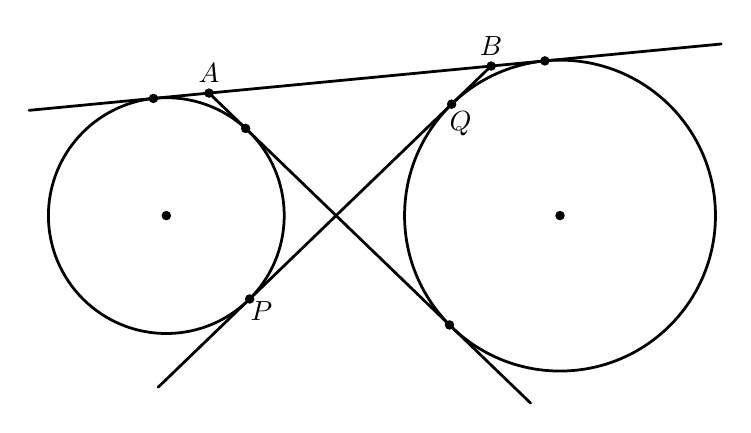
\begin{tikzpicture}[line cap=round,line join=round,>=triangle 45,x=5.0cm,y=5.0cm]
\draw [line width=1.pt] (0.,0.) circle (5*0.29943568323608505cm);
\draw [line width=1.pt] (1.,0.) circle (5*0.3948448671767196cm);
\draw [line width=1.pt] (-0.020564860119318035,-0.43579237608808374)-- (0.825105978456794,0.37988658369898004);
\draw [line width=1.pt] (0.9255528724621118,-0.4765284175341249)-- (0.10847290624613003,0.3111790148272779);
\draw [line width=1.pt] (-0.3486400708669083,0.2673530701771678)-- (1.4093228407252973,0.43589867950764677);
\draw [fill=black] (0.,0.) circle (1.5pt);
\draw [fill=black] (1.,0.) circle (1.5pt);
\draw [fill=black] (0.9615242406392943,0.39296575560399466) circle (1.5pt);
\draw [fill=black] (-0.032758936612939486,0.2976383383689851) circle (1.5pt);
\draw [fill=black] (0.20154306981121067,0.2214545538166568) circle (1.5pt);
\draw [fill=black] (0.7193670828449719,-0.2777546308252312) circle (1.5pt);
\draw [fill=black] (0.7247273896882502,0.2830679408692495) circle (1.5pt);
\draw[color=black] (0.747273896882502,0.2330679408692495) node {$Q$};
\draw [fill=black] (0.21173300214546276,-0.21173300214546273) circle (1.5pt);
\draw[color=black] (0.24173300214546276,-0.24173300214546273) node {$P$};
\draw [fill=black] (0.10847290624613003,0.3111790148272779) circle (1.5pt);
\draw[color=black] (0.10847290624613003,0.3611790148272779) node {$A$};
\draw [fill=black] (0.825105978456794,0.37988658369898004) circle (1.5pt);
\draw[color=black] (0.825105978456794,0.42988658369898004) node {$B$};
\end{tikzpicture}

%(Shariguin)
\end{problema}














\begin{problema}
Por el punto $A$ de la cuerda com\'un $AB$ de dos circunferencias se ha trazado
una recta que cruza la primera circunferencia en el punto $C$ y la segunda en el punto
$D$. La tangente a la primera circunferencia en el punto $C$ y la tangente a la segunda
circunferencia en el punto $D$ concurren en el punto $M$. Demostrar que los puntos $M$,
$C$, $B$ y $D$ yacen en una circunferencia.

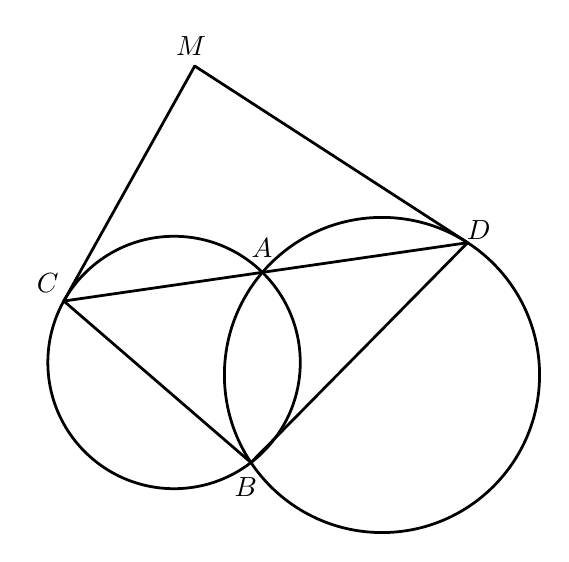
\begin{tikzpicture}[line cap=round,line join=round,>=triangle 45,x=0.85cm,y=0.85cm]
\draw [line width=1.pt] (0.7533333333333334,0.6333333333333332) circle (1.8857123617113807*0.85cm);
\draw [line width=1.pt] (3.86,0.4466666666666666) circle (2.3544190130239957*0.85cm);
\draw [line width=1.pt] (-0.8938882191430002,1.551250687003352)-- (1.9025873787892702,-0.8617005291976386);
\draw [line width=1.pt] (1.9025873787892702,-0.8617005291976386)-- (5.139529313030776,2.4230506440313566);
\draw [line width=1.pt] (-0.8938882191430002,1.551250687003352)-- (5.139529313030776,2.4230506440313566);
\draw [line width=1.pt] (-0.8938882191430002,1.551250687003352)-- (1.0627160912475522,5.062417326197354);
\draw [line width=1.pt] (1.0627160912475522,5.062417326197354)-- (5.139529313030776,2.4230506440313566);
\draw[color=black] (2.0666666666666678,2.3366666666666673) node {$A$};
\draw[color=black] (1.8266666666666675,-1.233333333333328) node {$B$};
\draw[color=black] (-1.1333333333333335,1.8166666666666673) node {$C$};
\draw[color=black] (5.306666666666669,2.6166666666666676) node {$D$};
\draw[color=black] (1.0066666666666673,5.356666666666667) node {$M$};
\end{tikzpicture}
%\\(GusievMIRclubsigma)

\end{problema}








\begin{problema}
Demostrar que la bisectriz del \'angulo recto de un tri\'angulo rect\'angulo divide
por la mitad el \'angulo entre la mediana y la altura bajadas sobre la hipotenusa.
%\\(SHARIGUIN I.35)

\vspace{3em}
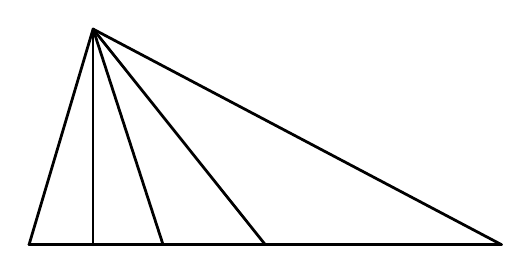
\begin{tikzpicture}[line cap=round,line join=round,>=triangle 45,x=6.0*.5cm,y=8.0*.5cm]
\draw [line width=1.pt] (-1.,0.)-- (1.,0.);
\draw [line width=1.pt] (-1.,0.)-- (-0.7289686274214113,0.6845471059286888);
\draw [line width=1.pt] (-0.7289686274214113,0.6845471059286888)-- (1.,0.);
\draw [line width=1.pt] (-0.7289686274214113,0.6845471059286888)-- (0.,0.);
\draw [line width=1.pt] (-0.7289686274214113,0.6845471059286888)-- (-0.7289686274214113,0.);
\draw [line width=1.pt] (-0.7289686274214113,0.6845471059286888)-- (-0.4327386422474257,0.);
\end{tikzpicture}

\end{problema}











\newpage
\begin{problema}
$AC$ y $BD$ son dos cuerdas de un círculo que se intersectan perpendicularmente. Mostrar que $|AD|^2+|BC|^2=4R^2$

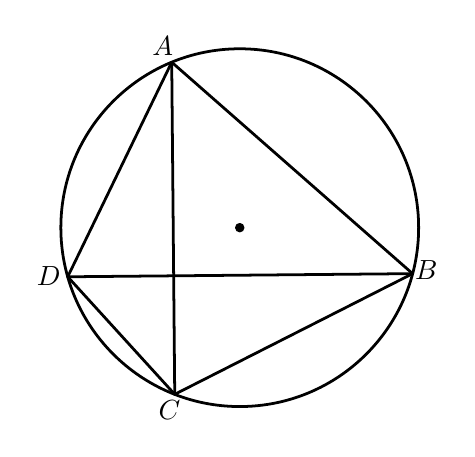
\begin{tikzpicture}[line cap=round,line join=round,>=triangle 45,x=3*0.8cm,y=3*0.8cm]
\draw [line width=1.0pt] (0.,0.) circle (3*0.9466241368757571*0.8cm);
\draw [line width=1.0pt] (-0.35996766036205713,0.875511587592785)-- (-0.34400569721099433,-0.8819055146681813);
\draw [line width=1.0pt] (0.9148148148148132,-0.243333333333333)-- (-0.9102440466537763,-0.2599096613193323);
\draw [line width=1.0pt] (-0.35996766036205713,0.875511587592785)-- (-0.9102440466537763,-0.2599096613193323);
\draw [line width=1.0pt] (-0.35996766036205713,0.875511587592785)-- (0.9148148148148132,-0.243333333333333);
\draw [line width=1.0pt] (0.9148148148148132,-0.243333333333333)-- (-0.34400569721099433,-0.8819055146681813);
\draw [line width=1.0pt] (-0.34400569721099433,-0.8819055146681813)-- (-0.9102440466537763,-0.2599096613193323);
\draw [fill=black] (0.,0.) circle (1.5pt);
\draw[color=black] (0.9870370370370354,-0.22388888888888858) node {$B$};
\draw[color=black] (-0.40740740740740883,0.9594444444444444) node {$A$};
\draw[color=black] (-0.3718518518518533,-0.9661111111111107) node {$C$};
\draw[color=black] (-1.0107407407407423,-0.2572222222222219) node {$D$};
\end{tikzpicture}
\end{problema}









\begin{problema}
En un triángulo equilátero $ABC$ se toman puntos $K$ en $AC$ y $M$ en $AB$ tales que las proporciones $AK:KC$ y $BM:MA$ son $2:1$. Mostrar que la longitud del segmento $KM$ es igual al radio del circuncírculo de $ABC$.  

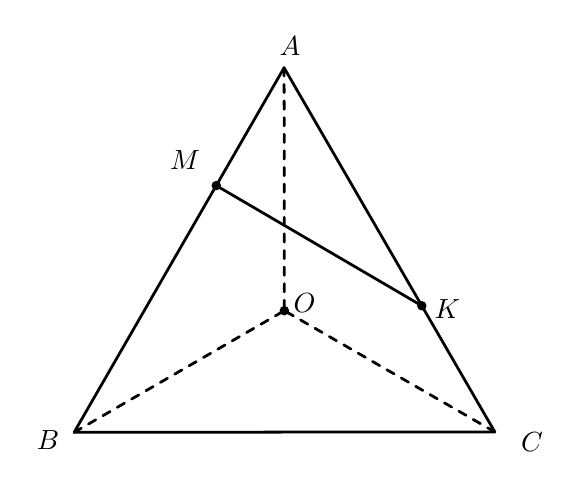
\begin{tikzpicture}[line cap=round,line join=round,>=triangle 45,x=15*1.0cm,y=15*1.0cm]
\draw [line width=1.pt] (0.34320987654320867,-0.17975308641975254)-- (0.6993905567235906,-0.17939217054933193);
\draw [line width=1.pt] (0.5209876543209864,0.12888888888888916)-- (0.6993905567235906,-0.17939217054933193);
\draw [line width=1.pt] (0.34320987654320867,-0.17975308641975254)-- (0.5209876543209864,0.12888888888888916);
\draw [line width=1.pt] (0.637593529145274,-0.07260661451065223)-- (0.46354242495975917,0.02915758791453644);
\draw [dashed, line width=1.pt](0.34320987654320867,-0.17975308641975254)--(0.5211960291959286,-0.0767521226933984);
\draw [dashed, line width=1.pt](0.6993905567235906,-0.17939217054933193)--(0.5211960291959286,-0.0767521226933984);
\draw [dashed, line width=1.pt](0.5209876543209864,0.12888888888888916)--(0.5211960291959286,-0.0767521226933984);
\draw[color=black] (0.5259259259259247,0.14703703703703727) node {$A$};
\draw[color=black] (0.3211728395061717,-0.18592592592592538) node {$B$};
\draw[color=black] (0.7308641975308628,-0.1883950617283945) node {$C$};
\draw [fill=black] (0.637593529145274,-0.07260661451065223) circle (1.5pt);
\draw[color=black] (0.6592592592592579,-0.07530864197530822) node {$K$};
\draw [fill=black] (0.46354242495975917,0.02915758791453644) circle (1.5pt);
\draw[color=black] (0.4370987654320976,0.05098765432098799) node {$M$};
\draw [fill=black] (0.5211960291959286,-0.0767521226933984) circle (1.5pt);
\draw[color=black] (0.5382716049382704,-0.07) node {$O$};
\end{tikzpicture}
%(Shariguin)
\end{problema}














\begin{problema}
%[OMM '99]
Sea ABCD un trapecio con $AB$ paralela a $CD$. Las bisectrices exteriores a los ángulos $B$ y $C$ se intersectan en $P$. Las bisectrices exteriores a los ángulos $A$ y $D$ se intersectan en $Q$. Mostrar que $|PQ|$ es igual a la mitad del perímetro de $ABCD$.  

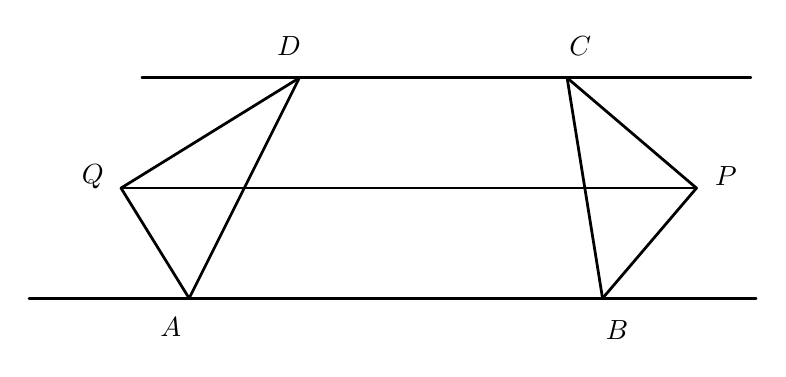
\begin{tikzpicture}[line cap=round,line join=round,>=triangle 45,x=2.5cm,y=2.5cm]
\draw [line width=1.pt] (0.3,0.)-- (2.4,0.);
\draw [line width=1.pt] (2.4,0.)-- (2.22,1.12);
\draw [line width=1.pt] (2.22,1.12)-- (0.86,1.12);
\draw [line width=1.pt] (0.86,1.12)-- (0.3,0.);
\draw [line width=1.pt] (-0.5133333333333334,0.)-- (0.3,0.);
\draw [line width=1.pt] (0.3,0.)-- (-0.046099033699941165,0.56);
\draw [line width=1.pt] (-0.046099033699941165,0.56)-- (0.86,1.12);
\draw [line width=1.pt] (0.06,1.12)-- (0.86,1.12);
\draw [line width=1.pt] (2.22,1.12)-- (3.1533333333333333,1.12);
\draw [line width=1.pt] (2.22,1.12)-- (2.8771860364994892,0.56);
\draw [line width=1.pt] (2.8771860364994892,0.56)-- (2.4,0.);
\draw [line width=1.pt] (2.4,0.)-- (3.18,0.);
\draw [line width=1.pt] (-0.046099033699941165,0.56)-- (2.8771860364994892,0.56);
\draw[color=black] (0.2066666666666667,-0.14666666666666517) node {$A$};
\draw[color=black] (2.4733333333333336,-0.16) node {$B$};
\draw[color=black] (2.2866666666666666,1.28) node {$C$};
\draw[color=black] (0.8066666666666668,1.28) node {$D$};
\draw[color=black] (-0.19,0.62) node {$Q$};
\draw[color=black] (3.026666666666667,0.62) node {$P$};
\end{tikzpicture}
%Sug: excírculos.
%\\(P5 omm 1999)
\end{problema}















\begin{problema}
Por el vértice $A$ de un triángulo $ABC$ se traza una recta paralela a $BC$. En esta paralela se toma el punto $D$ de manera que $|AD|=|AC|+|AB|$. El segmento $DB$ corta al lado $AC$ en el punto $E$. Demostrar que la recta por $E$ paralela a $BC$ pasa por el incentro de $ABC$.

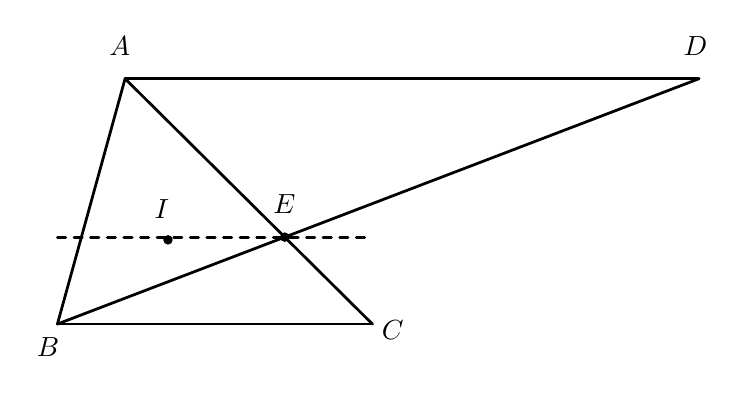
\begin{tikzpicture}[line cap=round,line join=round,>=triangle 45,x=4.0cm,y=4.0cm]
\draw [line width=1.pt] (0.,0.)-- (1.,0.);
\draw [line width=1.pt] (1.,0.)-- (0.21481481481481332,0.7788888888888885);
\draw [line width=1.pt] (0.21481481481481332,0.7788888888888885)-- (0.,0.);
\draw [line width=1.pt] (0.21481481481481332,0.7788888888888885)-- (2.0370370370370354,0.7788888888888885);
\draw [line width=1.pt] (0.,0.)-- (2.0370370370370354,0.7788888888888885);
\draw [dashed, line width=1.pt] (0.,0.27598425196850385)-- (1.,0.27598425196850385);
\draw[color=black] (-0.029629629629631102,-0.07388888888888859) node {$B$};
\draw[color=black] (1.064814814814813,-0.020555555555555792) node {$C$};
\draw[color=black] (0.19814814814814666,0.8816666666666663) node {$A$};
\draw[color=black] (2.0259259259259244,0.8816666666666663) node {$D$};
\draw [fill=black] (0.7217847769028866,0.27598425196850385) circle (1.5pt);
\draw[color=black] (0.7203703703703688,0.3816666666666666) node {$E$};
\draw [fill=black] (0.35099614201065826,0.26729704771206114) circle (1.5pt);
\draw[color=black] (0.33148148148148,0.365) node {$I$};
\end{tikzpicture}

\end{problema}

















\newpage
\begin{problema}
En una circunferencia de radio $R$ se traza un diámetro, sobre el que se elige un punto $A$, a distancia $a$ del centro. Si $r$ es el radio de la circunferencia pequeña que es tangente interior al círculo original y al diámetro en el punto $A$. Muestra que $r=\frac{R^2-a^2}{2R}$.

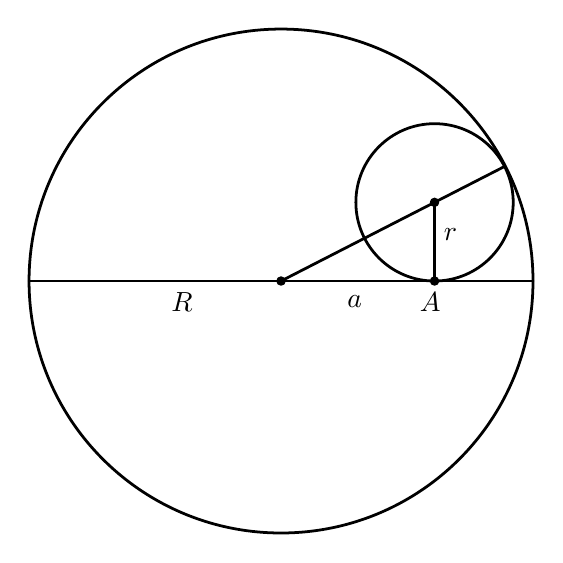
\begin{tikzpicture}[line cap=round,line join=round,>=triangle 45,x=4*0.8cm,y=4*0.8cm]
\draw [line width=1.pt] (0.,0.) circle (4*0.8cm);
\draw [line width=1.pt] (0.6092592592592577,0.31222222222222223) circle (4*0.31222222222222223*0.8cm);
\draw [line width=1.pt] (-1.,0.)-- (1.,0.);
\draw [line width=1.pt] (0.,0.)-- (0.8811223424149164,0.4515417231950009);
\draw [line width=1.pt] (0.6092592592592577,0.31222222222222223)-- (0.6092592592592577,0.);
\draw [fill=black] (0.,0.) circle (1.5pt);
\draw [fill=black] (0.6092592592592577,0.) circle (1.5pt);
\draw[color=black] (0.292592592592591,-0.08277777777777749) node {$a$};
\draw[color=black] (0.592592592592591,-0.08277777777777749) node {$A$};
\draw[color=black] (-0.392592592592591,-0.08277777777777749) node {$R$};
\draw[color=black] (0.672592592592591,0.18277777777777749) node {$r$};
\draw [fill=black] (0.6092592592592577,0.31222222222222223) circle (1.5pt);
\end{tikzpicture}
\end{problema}




















\begin{problema}
En el cuadrilátero $ABCD$, $O$ es el punto de intersección de las diagonales $AC$ y $BD$; $M$ un punto en $AC$ tal que $|AM|=|OC|$; $N$ un punto en $BD$ tal que $|BN|=|OD|$; $K$ y $L$ son los puntos medios de $AC$ y $BD$. Muestra que as rectas $ML$, $NK$ y la recta que une los gravicentros de $ABC$ y $ACD$ concurren.

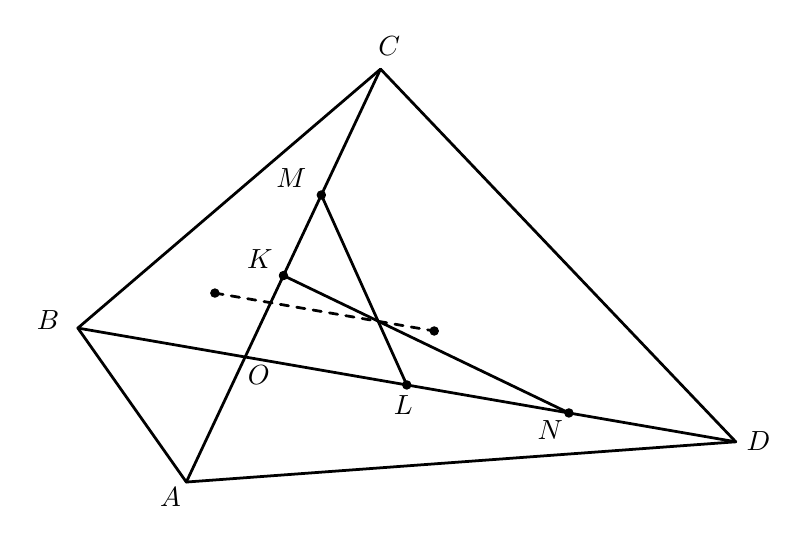
\begin{tikzpicture}[line cap=round,line join=round,>=triangle 45,x=4.0cm,y=4.0cm]
\draw [line width=1.pt] (2.0981481481481463,-0.8655555555555551)-- (0.009259259259257784,-0.504444444444444);
\draw [line width=1.pt] (0.3537037037037022,-0.9933333333333328)-- (0.9703703703703688,0.31777777777777794);
\draw [line width=1.pt] (0.009259259259257784,-0.504444444444444)-- (0.9703703703703688,0.31777777777777794);
\draw [line width=1.pt] (0.9703703703703688,0.31777777777777794)-- (2.0981481481481463,-0.8655555555555551);
\draw [line width=1.pt] (0.009259259259257784,-0.504444444444444)-- (0.3537037037037022,-0.9933333333333328);
\draw [line width=1.pt] (0.3537037037037022,-0.9933333333333328)-- (2.0981481481481463,-0.8655555555555551);
\draw [line width=1.pt] (0.6620370370370354,-0.33777777777777745)-- (1.568350086027346,-0.773968124603821);
\draw [line width=1.pt] (0.78235217883982,-0.0819726114223075)-- (1.053703703703702,-0.685);
\draw [dashed, line width=1.pt] (0.4444444444444429,-0.3933333333333329)--(1.1407407407407393,-0.5137037037037034);
\draw[color=black] (0.3037037037037022,-1.040555555555555) node {$A$};
\draw[color=black] (-0.08518518518518665,-0.47944444444444406) node {$B$};
\draw[color=black] (0.9981481481481465,0.390) node {$C$};
\draw[color=black] (2.1703703703703687,-0.8627777777777773) node {$D$};
\draw[color=black] (0.5837037037037023,-0.655) node {$O$};
\draw [fill=black] (0.78235217883982,-0.0819726114223075) circle (1.5pt);
\draw[color=black] (0.6870370370370356,-0.02944444444444419) node {$M$};
\draw [fill=black] (0.6620370370370354,-0.33777777777777745) circle (1.5pt);
\draw[color=black] (0.5870370370370355,-0.285) node {$K$};
\draw [fill=black] (1.568350086027346,-0.773968124603821) circle (1.5pt);
\draw[color=black] (1.5092592592592575,-0.8272222222222218) node {$N$};
\draw [fill=black] (1.053703703703702,-0.685) circle (1.5pt);
\draw[color=black] (1.042592592592591,-0.749444444444444) node {$L$};
\draw [fill=black] (0.4444444444444429,-0.3933333333333329) circle (1.5pt);
\draw [fill=black] (1.1407407407407393,-0.5137037037037034) circle (1.5pt);
\end{tikzpicture}
\end{problema}


















\begin{problema}
Sea $H$ el ortocentro de un triángulo, $D$ el punto medio de uno de los lados. $K$ uno de los puntos de intersección  de la recta $HD$ con el circuncírculo (de forma que $D$ se encuentra entre $H$ y $K$). Muestra que $D$ es el punto medio del segmento $HK$

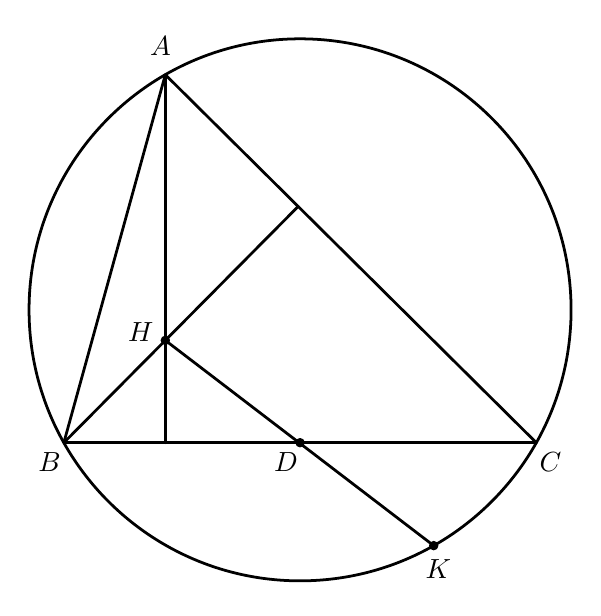
\begin{tikzpicture}[line cap=round,line join=round,>=triangle 45,x=6*1.0cm,y=6*1.0cm]
\draw [line width=1.pt] (0.5,0.28116878885542734) circle (6*0.5736339318994544cm);
\draw [line width=1.pt] (0.,0.)-- (1.,0.);
\draw [line width=1.pt] (1.,0.)-- (0.21481481481481332,0.7788888888888885);
\draw [line width=1.pt] (0.21481481481481332,0.7788888888888885)-- (0.,0.);
\draw [line width=1.pt] (0.21481481481481332,0.2165513111780339)-- (0.7828120506503471,-0.2179035824830124);
\draw [line width=1.pt] (0.21481481481481332,0.7788888888888885)-- (0.21481481481481332,0.);
\draw [line width=1.pt] (0.,0.)-- (0.49597449099804536,0.4999837950146736);
\draw[color=black] (0.20481481481481332,0.8388888888888885) node {$A$};
\draw[color=black] (-0.03,-0.04) node {$B$};
\draw[color=black] (1.03,-0.04) node {$C$};
\draw [fill=black] (0.21481481481481332,0.2165513111780339) circle (1.5pt);
\draw[color=black] (0.1625925925925911,0.235) node {$H$};
\draw [fill=black] (0.5,0.) circle (1.5pt);
\draw[color=black] (0.47037037037036883,-0.04055555555555527) node {$D$};
\draw [fill=black] (0.7828120506503471,-0.2179035824830124) circle (1.5pt);
\draw[color=black] (0.792592592592591,-0.2683333333333329) node {$K$};
\end{tikzpicture}
\end{problema}






































































\end{document}
